\smalltitle{سوال 1}
\begin{enumerate}
    \item به صورت کاردینالی به صورت زیر نشان داده می‌شود:
    \begin{figure}[H]
        \centering 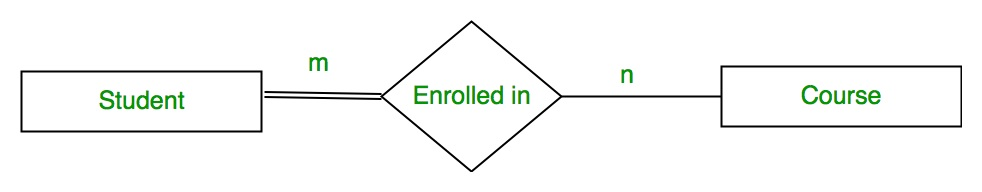
\includegraphics[scale=0.4]{pics/nullable1.jpg}
    \end{figure}
    تک خط که بین
    \lr{Enrolled in} و \lr{Course}
    نشان دهنده‌ی اختیاری بودن آن رابطه است. به عنوان مثال در اینجا این دیاگرام نشان دهنده‌ی این است
    که هر درس می‌تواند توسط تعدادی دانشجو اخذ شده باشد یا نه. این یعنی درسی می‌تواند خالی بماند.

    \noindent
    برای نشانه گذاری کمینه و بیشینه می‌توان به صورت زیر عمل کرد:
    \begin{figure}[H]
        \centering 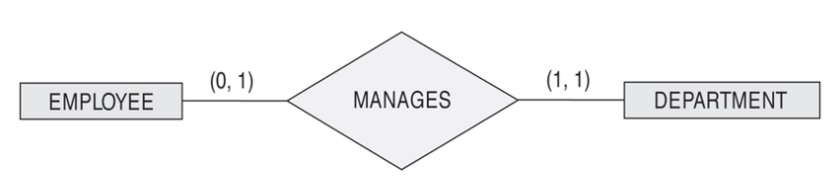
\includegraphics[scale=0.4]{pics/nullable2.jpg}
    \end{figure}
    در این مثال هر کارمند می‌تواند 1 یا 0 بخش را مدیریت کند ولی هر بخش حتما توسط یک نفر مدیریت می‌شود.
    \item \textbf{فایل}:
    \begin{enumerate}
        \item سادگی در ذخیره‌سازی فایل
    \end{enumerate}
    \textbf{پایگاه داده}:
    \begin{enumerate}
        \item کمتر کردن تکرار به کمک رابطه‌ها
        \item ارتباط تحت شبکه. این موضوع کمک می‌کند که برنامه‌ اصلی و دیتابیس را در دو کامپیوتر مختلف اجرا کنیم
        \item امکان درخواست (کوئری) زدن‌های پیچیده
        \item هندل کردن اتوماتیک \lr{data race} در خود دیتابیس
    \end{enumerate}
    \item رابطه‌ی دانشجو و دپارتمان. هر دانشجو برای یک دپارتمان است ولی هر دپارتمان چندین دانشجو دارد.
    \item زمانی اتفاق می‌افتد که مدل سازی معنای ما نشان می‌دهد که رابطه‌ای بین دو موجودیت وجود داشته باشد ولی در مدل طراحی
    شده این رابطه وجود نداشته باشد. به زبان ساده‌تر زمانی که یک رابطه به صورت کامل مدل نمی‌شود.
    به عنوان مثال مدل زیر را در نظر بگیرید:
    \begin{figure}[H]
        \centering 
\includegraphics[scale=0.25]{pics/1-4.png}
    \end{figure}
    در نگاه اول شاید مشکلی وجود نداشته باشد ولی فرض کنید که می‌خواهیم یک آزمایشگاه جدید اضافه کنیم. با این
    مدلسازی حتما باید کسی را سرپرست این آزمایشگاه قرار دهیم که بتوانیم آنرا در دپارتمانی قرار دهیم.
    در صورتی که اگر مدلسازی را به صورت زیر انجام می‌دادیم این مشکل پیش نمی‌آمد:
    \begin{figure}[H]
        \centering 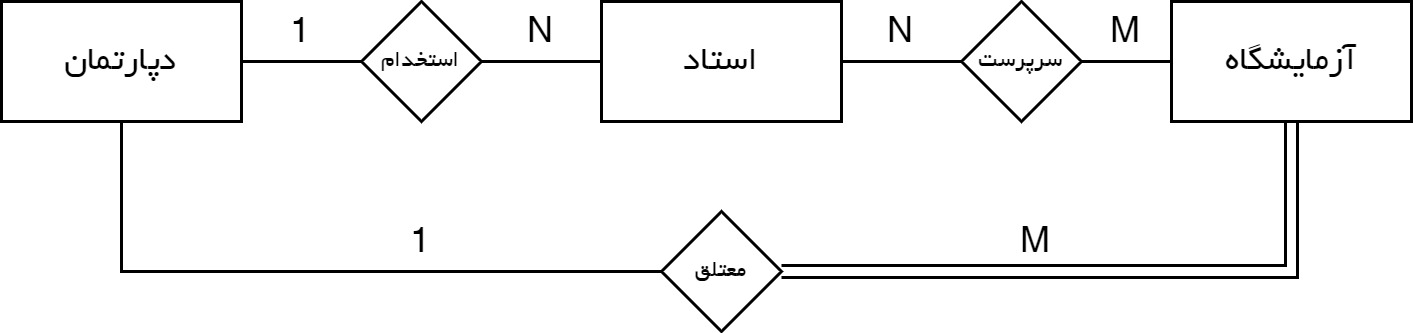
\includegraphics[scale=0.25]{pics/1-4-Fixed.png}
    \end{figure}
    % https://youtu.be/p4o5VrHoHcM
\end{enumerate}



